\documentclass[12pt,a4paper]{article} %report has annoying numbering habits
\usepackage{mystyle}
\usepackage{graphicx}
\usepackage{minted}
\usepackage{listings}
\usepackage[margin=1in]{geometry}
\usepackage{pdflscape}
\usepackage{pdfpages}
\usepackage{float}
\usepackage{flafter}
%\usemintedstyle{monokai}
\usepackage{auto-pst-pdf}

\title{Principles of Scientific Computing Homework 5}
\author{Michal Jander, Yevginiy Krasnitskiy, Jordan Palamos, and Andrea Yocom}
 
\begin{document}
 
\maketitle	
\tableofcontents
% \listoffigures
% \listoftables

\section{Instructions}
\begin{enumerate}
\item Get the data file
\item Average the 3 months and differentiate this curve in 5 year intervals. Plot the resulting slope vectors. Use a finite element approach or another way.
\item Use a numerical integration technique to compute the total area of the curve from 1870 to 1950 - compare that to the area under the curve from 1950 to 2013
\item Smooth the waveform in three ways, plot the three waveforms on the same graph and comment on differences in smoothing. Use the following methods:
	\begin{itemize}
	\item boxcar of width 5 years
	\item gaussian kernel of width 5 years
	\item exponential smoothing with greatest weight given to last 20 years
	\end{itemize}
\item Plot histogram of yearly ratios of July and Sept sea ice extent, comment on patterns
\item Window the data and baseline (polynomial fit ok) to extract two cooling periods prior to 1950 that allow sea extent to remain larger than average. Determine the total area of each event, compare to average area from period 1870 to 1950 to determine overall amplitude of cooling.
\item When is meltdown? Use two sets of data:
  a) entire data set, determine smooth functional form that best fits data, extrapolate to zero. Do not use polynomial fit in this case. Graph fitted line to the data, extrapolated to zero.
  b) use only September satellite data. Fit linear regression to the data, also some power or exponential law. Plot two fits on same graph.
\end{enumerate}


\section{Plotting, averaging, and finding the rate of change of Arctic Sea ice extent}

\subsection{General trends}
\paragraph{}
Figure \ref{avg_area_annual}, the 1870-2013 Arctic Sea ice extent averaged over the summer months (July, August, and September), illustrates that the arctic sea ice has dropped precipitously in the last 20 years, as compared to the approximately stable extent for the one hundred years preceding this. If we look at the months separately (as in Fig. \ref{months}), we see that the general trend is for July extent to be about one square kilometer above the average, the August extent to be about average, and the September extent about one square kilometer below the average.  

\begin{figure}[hbp]
\centering
 \includegraphics[width=0.75\linewidth]{../output/avg_area_annual.png}
\caption{Here you see a precipitous arctic sea ice extent drop starting in about 1980}
\label{avg_area_annual}
\end{figure}

\begin{figure}[hbp]
\centering
 \includegraphics[width=0.75\linewidth]{../img/iceExt.png}
\caption{July above average, August is average, and September is below average}
\label{months}
\end{figure}

\subsection{Sea ice extent change from 1870 to 1950 and from 1950 to 2013}
\paragraph{}
Averaging the summer month ice extent in five year bins as in Fig. \ref{avg_area_five_year} smooths things out a bit. Differentiating the curve shown in Fig. \ref{avg_area_five_year} in five year intervals yields a rate of change profile, shown in Fig. \ref{slope}. While pre-1950 ice extent changes seem to be roughly evenly distributed about zero, it is clear that after 1950 the ice extent changes begin trending steadily toward ice loss, with the most dramatic loss from 2000-2005. Integrating under the curve shown in Fig. \ref{slope} gives us a value for the total change in extent.
From 1870 to 1950, average ice extent increased by $0.166 km^{2}$. From 1950 to 2013, average ice extent decreased by $3.055 km^{2}$. 

\begin{figure}[hbp]
\centering
 \includegraphics[width=0.75\linewidth]{../output/avg_area_five_year.png}
\caption{A smoother version of sea ice extent loss}
\label{avg_area_five_year}
\end{figure}

\begin{figure}[hbp]
\centering
 \includegraphics[width=0.75\linewidth]{../output/slope.png}
\caption{Each five year stretch has some average rate of change in ice extent.}
\label{slope}
\end{figure}

\paragraph{}
We can plot this slope in a slightly different way. In Fig. \ref{spiky slope}, the slope is not plotted as a flat line. Numerically integrating under this curve using Simpson's rule yields different results.  Here, from 1870 to 1950, average ice extent increased by $0.03 km^{2}$. From 1950 to 2013, average ice extent decreased by $0.264 km^{2}$. The ratio of post-1950 loss to pre-1950 gain is $9.08$. This is about a ten-fold reduction. It seems that we are losing ten times more ice in the most recent 60 years than we've been able to accumulate in  the eighty years prior to that. 

\begin{figure}[hbp]
\centering
 \includegraphics[width=0.75\linewidth]{../img/iceGradient.png}
\caption{A different way to look at the slope.}
\label{spiky slope}
\end{figure}


\section{Smoothed sea ice extent data}
\paragraph{}
We use boxcar, Gaussian, and exponential smoothing techniques on the average ice data. 
The boxcar algorithm takes neighboring points and computes their average and replaces the middle point by the average.  We use five points with reflection on the endpoints (i.e. use the points near the endpoint reflected about the center point. 
\paragraph{}
The Gaussian algorithm replaces each point by the weighted average of the point and its neighbors, the weights being Gaussian distributed about the center point, with total of unity.  We use five points, with weights of $(0.067, 0.242, 0.383, 0.242, 0.067)$.
\paragraph{}
The exponential smoothing algorithm works according to Eqn. \ref{exp}, where $x(t)$ is the raw data,  $s(t)$ is the smoothed data, and $s(0) = x(0)$:
\begin{equation}
s(t) = a*x(t-1) + (1-a)*s(t-1).
\label{exp}
\end{equation}
The smoothing parameter $0<a<1$ works as follows:  Larger values of a give more weight to recent data but smoothing is worse. We use $a = 0.7$ to give greater weight to the more recent data but to keep the smoothing as good as possible.

\paragraph{}
All methods, shown in Fig. \ref{smoothed}, suppress local variations in favor of highlighting global variations. The boxcar and Gaussian smoothing techniques tend to be similar, and both methods lag the real data temporally. The exponential smoothing, on the other hand, leads the data temporally. It follows the raw data more closely than the boxcar or Gaussian methods, particularly the recent data. This was the intention of choosing a smoothing parameter close to unity. The fit is not as smooth as Gaussian or boxcar fits, but shows local variations better with reduced noise.

\begin{figure}[hp]
\centering
 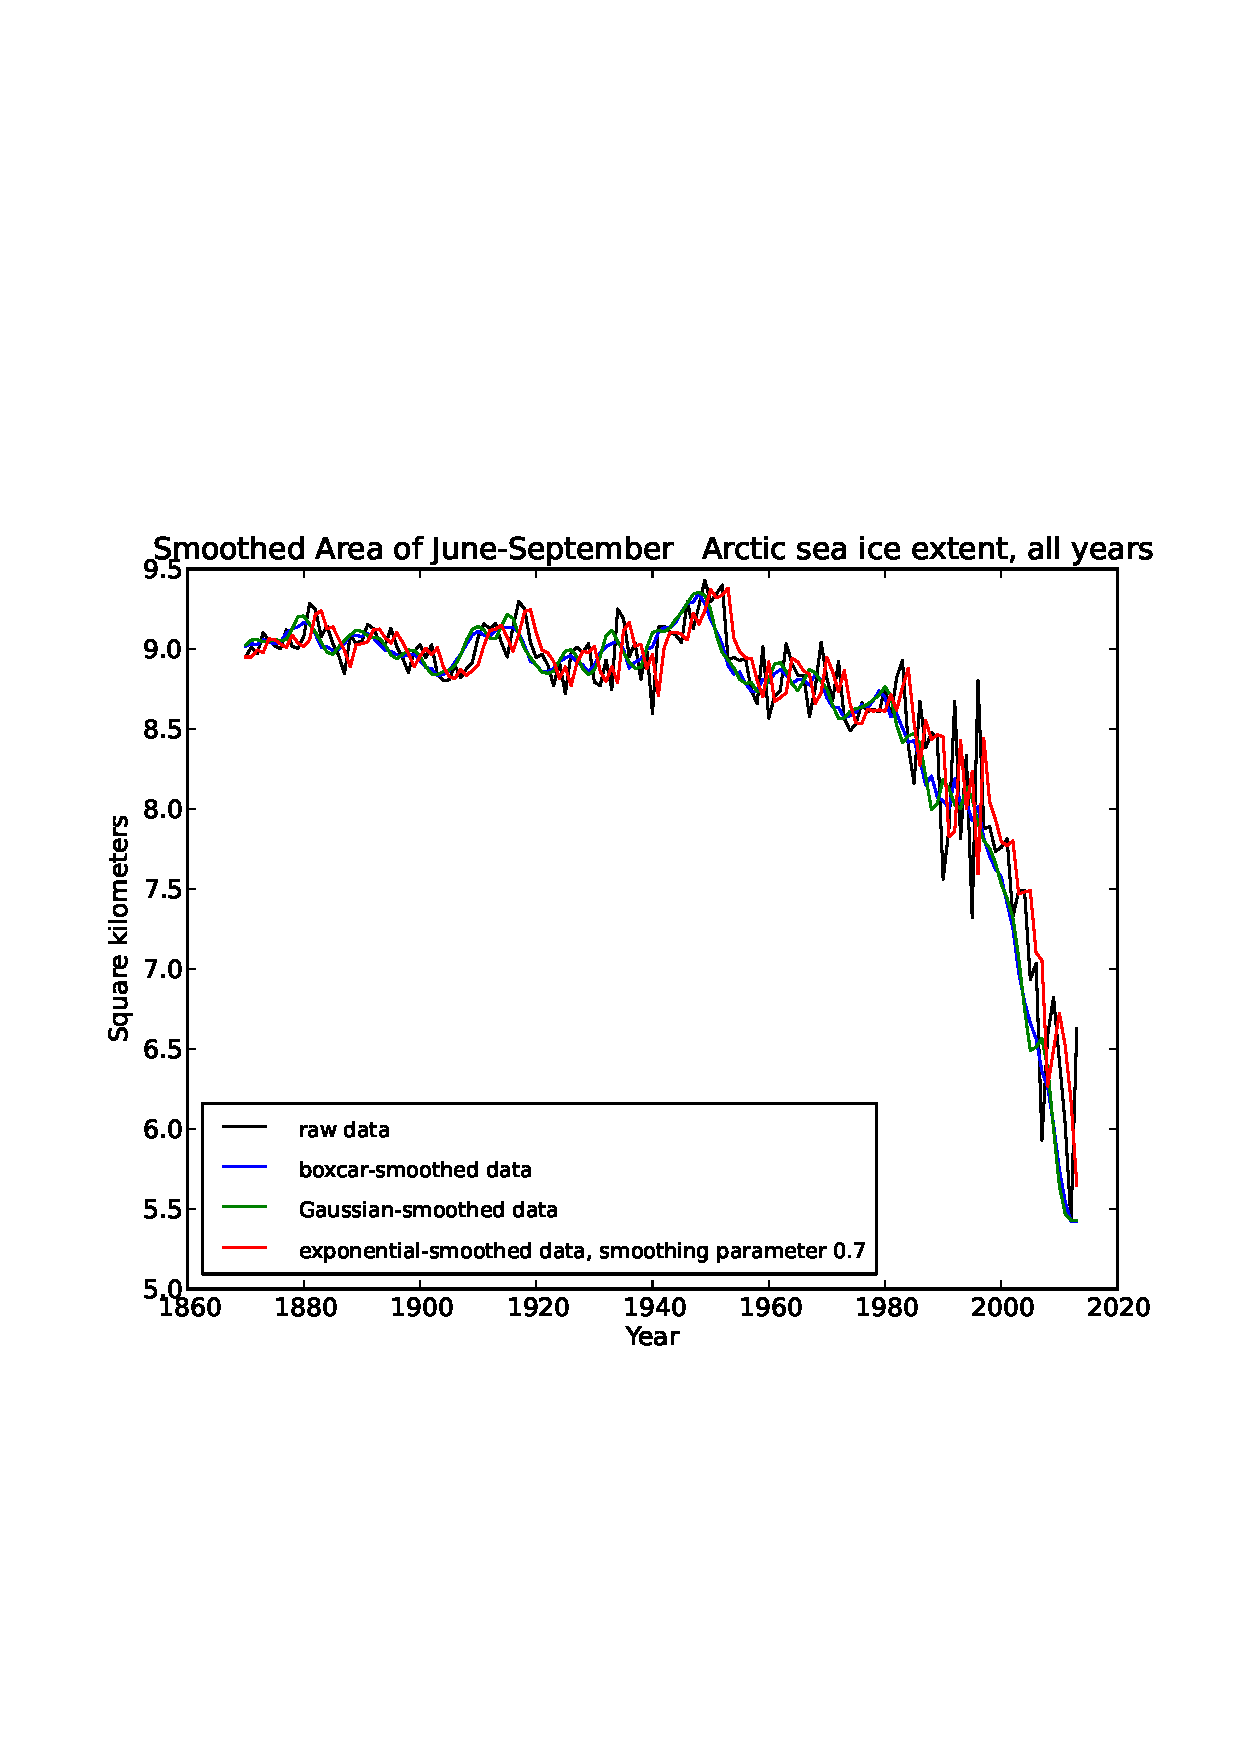
\includegraphics[width=0.75\linewidth]{../output/smooth_avg_area_annual.png}
\caption{Boxcar, Gaussian, and Exponential Smoothing comparisons}
\label{smoothed}
\end{figure}

\paragraph{}
To summarize the effects of the three smoothing methods: 
\begin{itemize}
\item Boxcar-smoothed data follows the global behavior of the raw data, but loses the local variations in the data.  It is the least noisy of the three.
\item Gaussian-smoothed data shows more of local variations than does boxcar-smoothed data, but the variations are not sharp and tend to be normally-smoothed-over.
\item Exponentially-smoothed data follows the local variations in the data much better, especially for the more recent data as was intended with the smoothing parameter, however the curve is not as smooth, still showing signs of noise.
\end{itemize}


\section{Histogram of summer melting events}
\paragraph{}Taking the ratio of July to September ice extent gives a measure of how much ice melted over the summer. The distribution, shown in Fig. \ref{hist} looks roughly Poissonian. The long tail may indicate some random events of large mass melting. The statistical significance of the large melting events is very small, however may still fall into the distribution of melting events that is depicted in the histogram.

\begin{figure}[!hbp]
\centering
 \includegraphics[width=0.75\linewidth]{../output/annual_ratio_hist.png}
\caption{Histogram of summer melting events}
\label{hist}
\end{figure}


\section{Pre-1950 cooling events}
\subsection{Attempt 1}
\paragraph{}
Looking at the events that have occurred prior to year 1950 we can find two windows of cooling periods for which the ice extent was above normal, shown in Fig. \ref{windows}. It looks like the first cooling period begins in 1933 and ends in 1936, and the second cooling period begins in 1945 and ends in 1953. We can compute the area under the gradient curves over these cooling periods and find the ratio to the total change in the sea ice extent (computed up to 1950). Using the first window from 1933 to 1936 and the second window from 1945 to 1950 (cooling periods) we find:
\begin{itemize}
\item change in extent of sea ice in first cooling window = $0.0453333333333$ square kilometers
\item change in extent of sea ice in the second cooling window = $0.164666666667$ square kilometers
\item ratio in first cooling window to total change prior to 1950 = $0.155873925501$
\item ratio in second cooling window to total change prior to 1950 = $0.566189111748$
\end{itemize}

\begin{figure}[hp]
\centering
 \includegraphics[width=0.75\linewidth]{../img/windowCooling.png}
\caption{Cooling period windows}
\label{windows}
\end{figure}

\subsection{Attempt 2}
\paragraph{}
If we consider the window from 1910-1920 we get a cooling magnitude of: 6.94 compared to an average cooling of: 2.46 for a relative cooling of: 4.48.
If we consider the window from 1940-1950 we get a cooling magnitude of: 3.250 compared to an average cooling of: 1.410 for a relative cooling of: 1.84.

\paragraph{}
Figures \ref{detrended}, \ref{baseline_fit}, and \ref{1940_removed} have some story but I don't know what it is yet.

\begin{figure}[hp]
\centering
 \includegraphics[width=0.75\linewidth]{../img/detrended.png}
\caption{Detrended Data}
\label{detrended}
\end{figure}

\begin{figure}[hp]
\centering
 \includegraphics[width=0.75\linewidth]{../img/baseline_fit.png}
\caption{A baseline fit}
\label{baseline_fit}
\end{figure}

\begin{figure}[hp]
\centering
 \includegraphics[width=0.75\linewidth]{../img/1940_removed.png}
\caption{1940 removed}
\label{1940_removed}
\end{figure}




\section{Extrapolation: visiting Santa via canoe}
\subsection{First attempt}
\paragraph{}Attempts to fit the entire data set with an exponential function did not succeed in finding the proper parameters. We can consider fitting a polynomial function to the entire data set.  This is accomplished in Fig. \ref{genepoly}  with a polynomial of degree 6. According to this fit, Arctic ice will melt completely by the year 2029.

\begin{figure}[hp]
\centering
 \includegraphics[width=0.75\linewidth]{../img/polyFitAllData.png}
\caption{Visit Santa by canoe in 2029}
\label{genepoly}
\end{figure}

\subsection{Fits to satellite data}
\paragraph{}
We can look at the data collected for the ice extent in September starting in the year 1979 and perform polynomial fits to the data to estimate the time at which Arctic sea ice will melt.  The linear (first degree polynomial) fit is shown in Fig. \ref{linfitsat}, and the  third degree polynomial fit is shown in Fig. \ref{polyFitSat}. Their predictions are stated in the figure captions.

\begin{figure}[hp]
\centering
 \includegraphics[width=0.75\linewidth]{../img/linearFitSat.png}
\caption{according to linear fit to satellite data Arctic ice will melt in the year 2067}
\label{linfitsat}
\end{figure}

\begin{figure}[hp]
\centering
 \includegraphics[width=0.75\linewidth]{../img/polyFitSat.png}
\caption{according to polynomial fit to satellite data Arctic ice will melt in the year 2028}
\label{polyFitSat}
\end{figure}

\newpage{}
\subsection{Another approach, using Matlab}
\includepdf[pages={-}]{../src/HW5_Part7.pdf}
%\include{../src/HW5_Part7.pdf}


\section{Code}
\paragraph{}
It can't really be argued that we truly collaborated here, given how all of us have our own code and own outputs. But we tried.
\subsection{Andrea's Code}
\input{../src/andrea_code.txt}
\subsection{Gene's Code}
\input{../src/gene_code.txt}
\subsection{Jordan's Code}
\input{../src/jordan_code.txt}

\end{document}